% !TEX root = ../CourseOT.tex

%%%%%%%%%%%%%%%%%%%%%%%%%%%%%%%%%%%%%%%%%%%%%%%%%%%%%%%%%%%%%%%%%%%%%%%%%%%
%%%%%%%%%%%%%%%%%%%%%%%%%%%%%%%%%%%%%%%%%%%%%%%%%%%%%%%%%%%%%%%%%%%%%%%%%%%
%%%%%%%%%%%%%%%%%%%%%%%%%%%%%%%%%%%%%%%%%%%%%%%%%%%%%%%%%%%%%%%%%%%%%%%%%%%
\section{Monge Problem between Measures}

%%%%%%%%%%%%%%%%%%%%%%%%%%%%%%%%%%%%%%%%%%%%%%%%%%%%%%%%%%%%%%%%%%%%%%%%%%%
\subsection{Measures}


%%%
\paragraph{Histograms}

We will interchangeably the term histogram or probability vector for any element $\a \in \simplex_n$ that belongs to the probability simplex
\eq{
	\simplex_n \eqdef \enscond{\a \in \RR_+^n}{ \sum_{i=1}^n \a_i = 1 }.
}


%%%
\paragraph{Discrete measure, empirical measure}

A discrete measure with weights $\a$ and locations $x_1,\dots,x_n\in\X$ reads
\eql{\label{eq-discr-meas}
	\al = \sum_{i=1}^n \a_i \de_{x_i}
}
where $\de_x$ is the Dirac at position $x$, intuitively a unit of mass which is infinitely concentrated at location $x$. Such as measure describes a probability measure if, additionally, $\a\in\simplex_n$, and more generally a positive measure if each of the ``weights'' described in vector $\a$ is positive itself. 
%
An ``empirical'' probability distribution is uniform on a point cloud, i.e. $\a=\frac{1}{n}\sum_i \de_{x_i}$. 
%
In practice, it many application is useful to be able to manipulate both the positions $x_i$ (``Lagrangian'' discretization) and the weights $\a_i$ (``Eulerian'' discretization). Lagrangian modification is usually more powerful (because it leads to adaptive discretization) but it breaks the convexity of most problems. 


%%%%
\paragraph{General measures}

We consider Borel measures $\al \in \Mm(\X)$ on a metric space $(\Xx,d)$, i.e. one can compute $\al(A)$ for any Borel set $A$ (which can be obtained by applying countable union, countable intersection, and relative complement to open sets). The measure should be finite, i.e. have a finite value on compact set.
%
A Dirac measure $\de_x$ is then define as $\de_x(A)=1$ is $x \in A$ and $0$ otherwise, and this extend by linearity for discrete measures of the form~\eqref{eq-discr-meas} as
\eq{
	\al(A) = \sum_{x_i \in A} \a_i  
}
%
We denote $\Mm_+(\X)$ the subset of all positive measures on $\X$, i.e. $\al(A) \geq 0$ (and $\al(\X)<+\infty$ for the measure to be finite). The set of probability measures is denoted $\Mm_+^1(\X)$, which means that any $\al \in \Mm_+^1(\X)$ is positive, and that $\al(\X)=1$. 


%%%%
\paragraph{Radon measures}

Using Lebesgue integration, a Borel measure can be used to compute integral of measurable functions (i.e. such that level sets $\enscond{x}{f(x) < t}$ are Borel sets), and we denote this pairing as
\eq{
	\dotp{f}{\al} \eqdef \int f(x) \d\al(x).
}
Integration of such a measurable $f$ against a discrete measure $\al$ computes a sum
\eq{ 
	\int_\X f(x) \d\al(x) = \sum_{i=1}^n \a_i f(x_i).
}

 
This can be in particular applied to the subspace of continuous functions which are measurable.
%
Integration against a finite measure on a compact space thus defines a continuous linear form $f \mapsto \int f \d\al$ on the Banach space of continuous functions $(\Cc(\Xx),\norm{\cdot}_\infty)$, indeed $|\int f \d\al| \leq \norm{f}_\infty |\al(\X)|$. 
%
On compact spaces, the converse is true, namely that any continuous linear form $\ell : f \mapsto \ell(f)$ on $(\Cc(\Xx),\norm{\cdot}_\infty)$ is represented as an integral against a measure $\ell(f)=\int f \d \al$. This is the  Riesz-Markov-Kakutani representation theorem, which is often stated that Borel measures can be identified to Radon measures.
%
Radon measures are thus in some sense ``less regular'' than functions, but more regular than distributions (which are dual to smooth functions). For instance, the derivative of a Dirac is not a measure.
%
This duality pairing $\dotp{f}{\al}$ between continuous function and measures will be crucial to develop duality theory for the convex optimization problem we will consider later. 

The associated norm, which is the norm of the linear form $\ell$, is the so-called total variation norm
\eq{
	\norm{\al}_{TV} = \norm{\ell}_{\Cc(\Xx)\rightarrow \RR} = \usup{f \in \Cc(\X)} \enscond{\dotp{f}{\al}}{ \norm{f}_\infty \leq 1 }.
}
(note that one can remove the $|\cdot|$ in the right hand side, and such a quantity is often called a ``dual norm'').
%
One can in fact show that this TV norm is the total mass of the absolute value measure $|\al|$.
%
The space $(\Mm(\Xx),\norm{\cdot}_{TV})$ is a Banach space, which is the dual of $(\Cc(\Xx),\norm{\cdot}_\infty)$. 

Recall that the absolute value of a measure is defined as 
\eq{
	|\al|(A) = \usup{A=\cup_i B_i} \sum_i |\al(B_i)|
}
so that for instance if $\al=\sum_i \a_i \de_{x_i}$, $|\al|=\sum_i |\a_i| \de_{x_i}$ and if $\d\al(x) = \rho \d x$ for a positif reference measure $\d x$, then $\d|\al|(x) = |\rho(x)| \d x$. 



%%%%%
\paragraph{Relative densities}

%TODO : ref measures
A measure $\al$ which is a weighting of another reference one $\d x$ is said to have a density, which is denoted $\d\al(x)=\density{\al}(x)\d x$  (on $\RR^d$ $\d x$ is often the Lebesgue measure), often also denoted $\density{\al} = \frac{\d\al}{\d x}$, which means that 
\eq{
	\foralls h \in \Cc(\RR^\dims), \quad
	\int_{\RR^\dims} h(x) \d\al(x) =  \int_{\RR^\dims} h(x) \density{\al}(x) \d x.
}

%%%%%
\paragraph{Probabilistic interpretation}

Radon probability measures can also be viewed as representing the distributions of random variables. A random variable $X$ on $\X$ is actually a map $X : \Om \rightarrow \X$ from some abstract (often un-specified) probabized space $(\Om,\PP)$, and its distribution is the Radon measure $\al \in \Mm_+^1(\X)$ such that $\PP(X \in A) = \al(A)=\int_A \d\al(x)$.


%%%%%%%%%%%%%%%%%%%%%%%%%%%%%%%%%%%%%%%%%%%%%%%%%%%%%%%%%%%%%%%%%%%%%%%%%%%
\subsection{Push Forward}
  
  
For some continuous map $\T : \X \rightarrow \Y$, we define the pushforward operator $\T_\sharp : \Mm(\X) \rightarrow \Mm(\Y)$. 
%
For a Dirac mass, one has $\T_\sharp \de_{x} = \de_{\T(x)}$, and this formula is extended to arbitrary measure by linearity. In some sense, moving from $\T$ to $\T_\sharp$ is a way to linearize any map at the prize of moving from a (possibly) finite dimensional space $\Xx$ to the infinite dimensional space $\Mm(\Xx)$, and this idea is central to many convex relaxation method, most notably Lasserre's relaxation.
%
For discrete measures~\eqref{eq-discr-meas}, the pushforward operation consists simply in moving the positions of all the points in the support of the measure
\eq{
	\T_{\sharp} \al \eqdef \sum_i \a_i \de_{\T(x_i)}.
}
For more general measures, for instance for those with a density, the notion of push-forward plays a fundamental to describe spatial modifications of probability measures. The formal definition reads as follow.

\begin{defn}[Push-forward]\label{defn-pushfwd}
For $\T : \X \rightarrow \Y$, the push forward measure $\be = \T_\sharp \al \in \Mm(\Y)$ of some $\al \in \Mm(\X)$ satisfies
\eql{\label{eq-push-fwd}
	\foralls h \in \Cc(\Y), \quad \int_\Y h(y) \d \be(y) = \int_\X h(\T(x)) \d\al(x).
	% = \int_X h(T(x)) \density{\al}(x) \d x %%%% y=T(x)   dy=|T'(x)| dx
	% = \int_Y h(y) \density{\al}(T^{-1}(y)) 1/|T'(x)| \d y 
	% = \int_Y h(y) \density{\be}(y) \d y
	%  \density{\al}(T^{-1}(y)) 1/|T'(x)| = \density{\be}(y)
}
Equivalently, for any measurable set $B \subset \Y$, one has
\eql{\label{eq-equiv-pushfwd}
	\be(B) = \al( \enscond{x \in \X}{\T(x) \in B} ).
}
Note that $\T_\sharp$ preserves positivity and total mass, so that if $\al \in \Mm_+^1(\X)$ then $\T_\sharp \al \in \Mm_+^1(\Y)$. 
\end{defn}

% Intuitively, a measurable map $T: \X\rightarrow \Y$, can be interpreted as a function ``moving'' a single point from a measurable space to another. The more general extension $T_\sharp$ can now ``move'' an entire probability measure on $\X$ towards a new probability measure on $\Y$. The operator $T_\sharp$ ``pushes forward'' each elementary mass of a measure $\al$ on $\X$ by applying the map $T$ to obtain then an elementary mass in $\Y$, to build on aggregate a new measure on $\Y)$ written $T_{\sharp}\al$.  Note that such a push-forward $\T_\sharp : \Mm_+^1(\X) \rightarrow \Mm_+^1(\Y)$ is a linear operator between measures in the sense that for two measures $\al_1,\al_2$ on $\X$, $T_\sharp(\al_1+\al_2)=T_\sharp\al_1+ T_\sharp\al_2$.



%%%%%%%
\begin{rem}[Push-forward for densities]
Explicitly doing the change of variable $x=T(x)$, so that $\d x = |\det(T'(x))| \d y$ in formula~\eqref{eq-push-fwd} for measures with densities $(\density{\al},\density{\be})$ on $\RR^\dims$ (assuming $\T$ is smooth and a bijection), one has for all $h \in \Cc(\Yy)$
\begin{align*}
	\int_\Yy h(y)\rho_\be(y) \d y &= \int_\Yy h(y) \d \be(y) = \int_\Xx h(T(x)) \d \al(x) = \int_\Xx h(T(x)) \rho_\al(x) \d x \\
		&= \int_\Yy h(y) \rho_\al(T^{-1}y) \frac{\d y}{|\det(T'( T^{-1} y))|}, 
\end{align*}
which shows that 
\eq{
	\rho_\be(y) = \rho_\al(T^{-1}y) \frac{1}{|\det(T'( T^{-1} y))|}.
}
Since $T$ is a diffeomorphism, one obtains equivalently
\eql{\label{eq-pfwd-density}
	\density{\al}(x) = |\det(\T'(x))|  \density{\be}(\T(x))
}
where $\T'(x) \in \RR^{\dims \times \dims}$ is the Jacobian matrix of $T$ (the matrix formed by taking the gradient of each coordinate of $T$).
%
This implies, denoting $y=\T(x)$
\eq{
	|\det(\T'(x))| = \frac{ \density{\al}(x) }{ \density{\be}(y) }.
}
\end{rem}
%%%%%%%


%%%%%%%%
%\begin{rem}[Push-forward vs. pull-back]
%The push-forward $\T_\sharp$ of measures should not be confounded with the pull-back of function $\T^\sharp : \Cc(\Y) \rightarrow \Cc(\X)$ which corresponds to the ``warping'' of functions. It is the linear map defined, for $g \in \Cc(\Y)$ by $\T^\sharp g = g \circ \T$. Push-forward and pull-back are actually adjoint one from each others, in the sense that
%\eq{
%	\foralls (\al,g) \in \Mm(\X) \times \Cc(Y), \quad
%	\int_\Y g \d( \T_\sharp\al ) = \int_\X (\T^\sharp g) \d\al.
%}
%It is important to realize that even if $(\al,\be)$ have densities $(\density{\al},\density{\be})$, $\T_\sharp \al$ is not equal to $\T^\sharp \density{\be}$, because of the presence of the Jacobian in~\eqref{eq-pfwd-density}.
%%
%This explains why OT should be used with caution to perform image registration, because it does not operate as an image warping method.
%%
%Figure~\ref{fig-push-pull} illustrate the distinction between these push-forward and pull-back operators. 
%\end{rem}
%%%%%%%%


%\begin{figure}
%\centering
%\begin{tabular}{@{}c@{\hspace{5mm}}c@{}}
%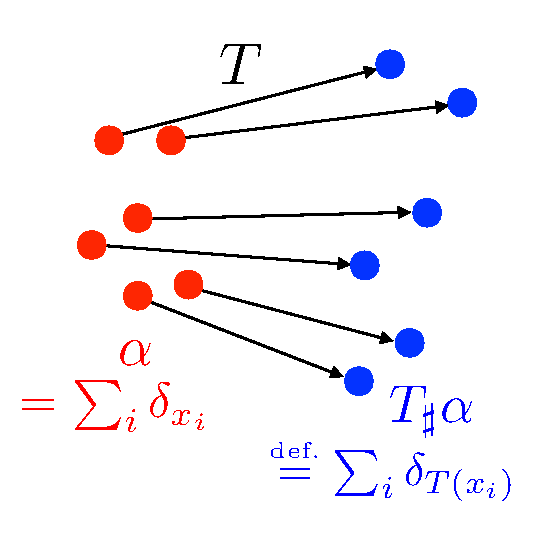
\includegraphics[width=.3\linewidth]{push-pull/push-forward}&
%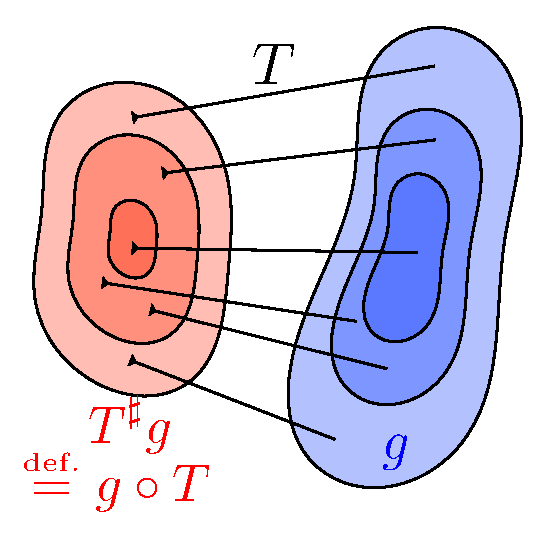
\includegraphics[width=.3\linewidth]{push-pull/pull-back}\\
%Push-forward of measures & Pull-back of functions
%\end{tabular}
%\caption{\label{fig-push-pull}
%Comparison of push-forward $\T_\sharp$ and pull-back $\T^\sharp$.
%}
%\end{figure}



\begin{rem}[Probabilistic interpretation]
A random variable $X$, equivalently, is the push-forward of $\PP$ by $X$, $\al=X_\sharp\PP$.
%
Applying another push-forward $\be = \T_\sharp\al$ for $\T : \X \rightarrow \Y$, following~\eqref{eq-push-fwd}, is equivalent to defining another random variable $Y=\T(X) : \om \in \Om \rightarrow \T(X(\om)) \in Y$, so that $\be$ is the distribution of $Y$.
%
Drawing a random sample $y$ from $Y$ is thus simply achieved by computing $y=\T(x)$ where $x$ is drawn from $X$. 
\end{rem}


%%%%%%%%%%%%%%%%%%%%%%%%%%%%%%%%%%%%%%%%%%%%%%%%%%%%%%%%%%%%%%%%%%%%%%%%%%%
\subsection{Monge's Formulation}


%%%%
\paragraph{Monge problem.}

Monge problem~\eqref{eq-optimal-assignment} is extended to the setting of two arbitrary probability measures $(\al,\be)$ on two spaces $(\X,\Y)$ as finding a map $\T : \X \rightarrow \Y$ that minimizes
\eql{\label{eq-monge-continuous}
	\uinf{\T} \enscond{ \int_{\X} \c(x,\T(x)) \d \al(x)  }{  \T_\sharp \al = \be }.
}
The constraint $\T_\sharp \al = \be$ means that $\T$ pushes forward the mass of $\al$ to $\be$, and makes use of the push-forward operator~\eqref{eq-push-fwd}. 

For empirical measure with same number $n=m$ of points, one retrieves the optimal matching problem. Indeed, this corresponds to the setting of empirical measures $\al=\sum_i \de_{x_i}$ and $\be=\sum_i \de_{y_i}$.  In this case, $\T_\sharp \al=\be$ necessarily implies that $\si$ is one-to-one, $\T : x_i \mapsto x_{\si(i)}$, so that 
\eq{
	\int_{\X} \c(x,\T(x)) \d \al(x) = \sum_i c(x_i,x_{\si(i)}).
}

In general, an optimal map $T$ solving~\eqref{eq-monge-continuous} might fail to exist. In fact, the constraint set $\T_\sharp \al = \be$, which is the case for instance if $\al=\de_x$ and $\be$ is not a single Dirac. 
%
Even if the constraint set is not empty the infimum might not be reached, the most celebrated example being the case of $\al$ being distributed uniformly on a single segment and $\be$ being distributed on two segments on the two sides.


%%%%
\paragraph{Monge distance.}

In the special case $c(x,y)=d^p(x,y)$ where $d$ is a distance, we denote 
\eql{\label{eq-monge-distance}
	\tilde\Wass_p^p(\al,\be) \eqdef 
		\uinf{\T} \enscond{ \Ee_\al(T) \eqdef \int_{\X} d(x,\T(x))^p \d \al(x)  }{  \T_\sharp \al = \be }.
}
If the constraint set is empty, then we set $\tilde \Wass_p^p(\al,\be) = +\infty$.
%
The following proposition shows that quantity defines a distance.

\begin{prop}
	$\tilde \Wass$ is a distance.
\end{prop}
\begin{proof}
	If $\tilde \Wass_p^p(\al,\be)=0$ then necessarily the optimal map is $\Id$ on the support of $\al$ and $\be=\al$.
	%
	Let us prove that $\tilde \Wass_p(\al,\be) \leq \tilde \Wass_p(\al,\ga)+\tilde \Wass_p(\ga,\be)$.
	If $\tilde \Wass_p(\al,\be)=+\infty$, then either $\tilde \Wass_p(\al,\ga)=+\infty$ or $\tilde \Wass_p(\ga,\be)=+\infty$, because otherwise we consider two maps $(S,T)$ such that $S_\sharp \al=\ga$ and $T_\sharp \ga=\be$ and then $(T \circ S)_\sharp \al = \be$ so that 
	$\tilde \Wass_p^p(\al,\be) \leq \Ee_\al(S \circ T) < +\infty$.
	%
	So necessarily $\tilde \Wass_p^p(\al,\be)<+\infty$ and we can restrict our attention to the cases 
	where $\tilde \Wass_p^p(\al,\ga)<+\infty$ and $\tilde \Wass_p^p(\ga,\be)<+\infty$ because otherwise the inequality is trivial.
	%
	For any $\epsilon>0$, we consider $\epsilon$-minimizer $S_\sharp \al=\ga$ and $T_\sharp \ga=\be$ such that
	\eq{
		E_\al(S)^{\frac{1}{p}} \leq \tilde \Wass_p(\al,\ga)+\epsilon
		\qandq
		E_\ga(T)^{\frac{1}{p}} \leq \tilde \Wass_p(\ga,\be)+\epsilon.
	}
	%
	Now we have that $(T \circ S)_\sharp \al=\ga$, so that 
	one has, using sub-optimality of this map and the triangular inequality 
	\eq{
		\Wass_p(\al,\ga) \leq \int d(x,T(S(x)))^p \d\al(x)^{\frac{1}{p}}
			\leq
			\int (d(x,S(x)) + d(S(x),T(S(x))))^p \d\al(x)^{\frac{1}{p}}	.		
	}
	The using Minkowski inequality for the $L^p$ spaces with measure $\al$ 
	\eq{
		\norm{f+g}_{L^p(\al)} \leq \norm{f}_{L^p(\al)} + \norm{g}_{L^p(\al)}
	}
	and with $f(x) \triangleq d(x,S(x))$ and $g(x) \triangleq d(S(x),T(S(x)))$
	one has
	\eq{
		\Wass_p(\al,\ga) \leq
			\int d(x,S(x))^p \d\al(x)^{\frac{1}{p}}	
			+ 		
			\int d(S(x),T(S(x)))^p \d\al(x)^{\frac{1}{p}}	
		\leq \Wass_p(\al,\be) + \Wass_p(\be,\ga) + 2 \epsilon.
	}
	Letting $\epsilon \rightarrow 0$ gives the result. 
\end{proof}

%%%%%%%%%%%%%%%%%%%%%%%%%%%%%%%%%%%%%%%%%%%%%%%%%%%%%%%%%%%%%%%%%%%%%%%%%%%
\subsection{Existence and Uniqueness of the Monge Map}

%%%%
\paragraph{Brenier's theorem.}

The following celebrated theorem of~\cite{Brenier91} ensures that in $\RR^\dims$ for $p=2$, if at least one of the two inputs measures has a density, then Kantorovitch and Monge problems are equivalent.

\begin{thm}[Brenier]\label{thm-brenier}
	In the case $\X=\Y=\RR^\dims$ and $c(x,y)=\norm{x-y}^2$, if $\al$ has a density with respect to the Lebesgue measure, then there exists a unique optimal Monge map $\T$. This map is characterized by being the unique gradient of a convex function $\T=\nabla \phi$ such that $(\nabla \phi)_\sharp \al = \be$. 
\end{thm}

Its proof requires to study the relaxed Kantorovitch problems and its dual, so we defer it to later (Section~\ref{sec-c-transfo}). 


%This results shows that in the setting of $\Wass_2$ with non-singular densities, the Monge problem~\eqref{eq-monge-continuous} and its Kantorovich relaxation~\eqref{eq-mk-generic} are equal (the relaxation is tight). This is the continuous analog of Proposition~\ref{prop-matching-kanto} for the assignment case~\eqref{prop-matching-kanto}, which states that the minimum of the optimal transport problem is achieved, when the marginals are equal and uniform, at a permutation matrix (a discrete map).
%
Brenier's theorem, stating that an optimal transport map must be the gradient of a convex function, should be examined under the light that a convex function is a natural generalization of the notion of increasing functions in dimension more than one. 
%
For instance, the gradient of a convex function is a monotone gradient field in the sense
\eq{
	\foralls (x,x') \in \RR^d \times \RR^d, \quad 
	\dotp{\nabla\phi(x)-\nabla\phi(x')}{x-x'} \geq 0.
}
Note however that in dimension larger than 1, not all monotone fields are gradient of convex function. For instance, a rotation is monotone but can never be an optimal transport because a gradient field $Ax$ defined by a linear map $A$ is necessarily obtained by a symmetric matrix $A$. Indeed, such a linear field must be associated to a quadratic form $\phi(x)=\dotp{Bx}{x}/2$
and hence $A=\nabla \phi = (B+B^\top)/2$.
%
Optimal transport can thus plays an important role to define quantile functions in arbitrary dimensions, which in turn is useful for applications to quantile regression problems~\cite{carlier2016vector}.
 

Note also that this theorem can be extended in many directions.  
% 
The condition that $\al$ has a density can be weakened to the condition that it does not give mass to ``small sets'' having Hausdorff dimension smaller than $\dims-1$ (e.g. hypersurfaces). 
%
One can also consider costs of the form $\c(x,y)=h(x-y)$ where $h$ is a strictly convex smooth function, for for instance $c(x,y)=\norm{x-y}^p$ with $1<p<+\infty$. 

Note that Brenier's theorem provides existence and uniqueness, but in general, the map $\T$ can be very irregular. 
%
Indeed, $\phi$ is in general non-smooth, but it is in fact convex and Lipschitz, so that $\nabla \phi$ is actually well defined $\al$-almost everywhere. Ensuring $\T$ to be smooth actually requires the target $\be$ to be regular, and  more precisely its support must be convex.

If $\al$ does not have a density, then $\T$ might fail to exists and it should be replaced by a set-valued function included in $\partial\phi$ which is now the sub-differential of a convex function, which might have singularity on a non-zero measure set. This means that $\T$ can ``split'' the mass by mapping to several locations  $T(x) \subset \partial\phi$. Actually, the condition that $T(x) \subset \partial\phi(x)$ and $\T_\sharp \al=\be$ implies that the multi-map $\T$ defines a solution of Kantorovitch problem that will be studied later. 



%%%%%%%
\paragraph{Monge-Amp\`ere equation.}

For measures with densities, using~\eqref{eq-pfwd-density}, one obtains that $\phi$ is the unique (up to the addition of a constant) convex function which solves the following Monge-Ampère-type equation
\eql{\label{eq-monge-ampere}
	\det(\partial^2\phi(x))  \density{\be}(\nabla\phi(x)) = \density{\al}(x)
}
where $\partial^2\phi(x) \in \RR^{\dims \times \dims}$ is the hessian of $\phi$. 
%
The convexity constraint forces $\det(\partial^2\phi(x)) \geq 0$ and is necessary for this equation to have a solution and be well-posed. 
%
The Monge-Amp\`ere operator $\det(\partial^2\phi(x))$ can be understood as a non-linear degenerate Laplacian. In the limit of small displacements, one can consider $\phi(x)=\norm{x}^2/2 + \epsilon\psi$ so that $\nabla \phi = \Id+\epsilon \nabla \psi$, one indeed recovers the Laplacian $\Delta$ as a linearization since for smooth maps
\eq{
	\det(\partial^2\phi(x)) = 1 + \epsilon \Delta \psi(x) + o(\epsilon), 
}
where we used the fact that $\det(\Id+\epsilon A) = 1+\epsilon\tr(A)+o(\epsilon)$. 



%%%%%%%
\paragraph{OT in 1-D.}

For a measure $\al$ on $\RR$, we introduce the cumulative function
\eql{\label{eq-cumul-defn}
	\foralls x \in \RR, \quad \cumul{\al}(x) \eqdef \int_{-\infty}^x \d\al, 
}
which is a function $\cumul{\al} : \RR \rightarrow [0,1]$.
%
Its pseudo-inverse  $\cumul{\al}^{-1} : [0,1] \rightarrow \RR \cup \{-\infty\}$ 
\eq{
	\foralls r \in [0,1], \quad \cumul{\al}^{-1}(r) = \umin{x} \enscond{x \in \RR \cup \{-\infty\} }{ \cumul{\al}(x) \geq r }.
}
That function is also called the quantile function of $\alpha$. 
%
The following proposition shows that these defines push-forward toward the uniform distribution $\Uu$ on $[0,1]$.

\begin{prop}
	One has $(\Cc_\al)^{-1}_\sharp \Uu = \al$,  
	where $\Uu$ is the uniform distribution in $[0,1]$. 
	%
	If $\al$ has a density, then $(\Cc_\al)_\sharp \al = \Uu$.
\end{prop}
\begin{proof}
	For simplicity, we assume $\al$ has a strictly positive density, so that $\Cc_\al$ is a strictly increasing continuous function.
	%
	Denoting $\ga \eqdef (\Cc_\al)^{-1}_\sharp \Uu$ we aim at proving $\ga=\al$, which is equivalent to 
	$\Cc_\ga=\Cc_\al$. One has
	\eq{
		\Cc_\ga(x) = \int_{-\infty}^x \d \ga = \int_\RR 1_{]-\infty,x]} \d( (\Cc_\al^{-1})_\sharp \Uu)
		  	 = \int_0^1 1_{]-\infty,x]}(\Cc_\al^{-1}(z)) \d z
			 = \int_0^1 1_{[0,\Cc_\al(x)]}(z) \d z
			 = \Cc_\al(x)
	}
	where we use the fact that 
	\eq{
		-\infty \leq \Cc_\al^{-1}(z) \leq x 
		\quad\Longleftrightarrow
		0 \leq z \leq \Cc_\al(x).
	}
\end{proof}

%
If $\al$ has a density, this shows that the map
\eql{\label{eq-OT-map-1d}
 	\T = \cumul{\be}^{-1} \circ \cumul{\al}
}
satisfies $\T_\sharp \al = \be$. 

For the cost $c(x,y)=|x=y|^2$, since this $\T$ is increasing (hence the gradient of a convex function since we are in 1-D), by Brenier's theorem, $\T$ is the solution to Monge problem (at least if we impose that $\al$ has a density, otherwise it might lead to a solution of Kantorovitch problem by properly defining the pseudo-inverse). 
%
This closed form formula is also optimal for any cost of the form $h(|x-y|)$ for increasing $h$. 
%
For discrete measures, one cannot apply directly this reasoning (because $\al$ does not have a density), but if the measure are uniform on the same number of Dirac masses, then this approach is actually equivalent to the sorting formula. 

Plugging this optimal map into the definition of the ``Wasserstein'' distance (we will see later that this quantity defines a distance), so that for any $p \geq 1$, one has
\eql{\label{eq-wass-cumul}
	\Wass_p(\al,\be)^p =
	\int_\RR |x- \cumul{\be}^{-1}( \cumul{\al}(x) )| \d \al(x)
	= \int_0^1 | \cumul{\al}^{-1}(r) - \cumul{\be}^{-1}(r) |^p \d r = 	
	 \norm{ \cumul{\al}^{-1} - \cumul{\be}^{-1} }_{L^p([0,1])}^p .
}
This formula is still valid for any measure (one can for instance approximate $\al$ by a measure with density). 
%
This formula means that through the map $\al \mapsto \cumul{\al}^{-1}$, the Wasserstein distance is isometric to a linear space equipped with the $L^p$ norm. For $p=2$, the Wasserstein distance for measures on the real line is thus a Hilbertian metric. 
This makes the geometry of 1-D optimal transport very simple, but also very different from its geometry in higher dimensions, which is not Hilbertian.

For $p=1$, one even has the simpler formula. Indeed, the previous formula is nothing more than the area between the two graphs of the copula, which can thus be computed by exchanging the role of the two axis, so that 
\begin{align}\label{eq-w1-1d}
	\Wass_1(\al,\be) &= \norm{ \cumul{\al} - \cumul{\be} }_{L^1(\RR)} = 
	\int_\RR | \cumul{\al}(x) - \cumul{\be}(x) | \d x 
	= \int_\RR \abs{ \int_{-\infty}^x \d(\al-\be) } \d x.
\end{align}
which shows that $\Wass_1$ is a norm (see paragraph \ref{sec-W1} for the generalization to arbitrary dimensions). 

It is possible to define other type of norm which behave similarly (i.e. metrize the convergence in law), for instance $\norm{ \cumul{\al} - \cumul{\be} }_{L^p(\RR)}$ define respectively the Wasserstein, Cramer (i.e. Sobolev) and Kolmogorov-Smirnov norms for $p=1,2,\infty$. 



% Figure~\ref{fig-1d-ot} illustrates the computation of 1-D OT through cumulative functions. It also displays displacement interpolations, computed as detailed in~\eqref{eq-displacement-1d-cumul}, see also Remark~\ref{rem-bary-1d}. For a detailed survey of the properties of optimal transport in 1-D, we refer the reader to~\cite[Chapter 2]{SantambrogioBook}.


%
%\newcommand{\MyFigCumulMeas}[1]{\includegraphics[width=.28\linewidth]{1d-cumulative/#1}}
%\newcommand{\MyFigCumulCum}[1]{\includegraphics[width=.2\linewidth]{1d-cumulative/#1}}
%\begin{figure}
%\centering
%\begin{tabular}{@{}c@{\hspace{1mm}}c@{\hspace{1mm}}c@{}}
%\MyFigCumulMeas{input-mu}&
%\MyFigCumulMeas{input-nu}&
%\MyFigCumulMeas{interp-bary}\\
%$\mu$ & $\nu$ & ${ (t\T+(1-t)\Id)_\sharp \mu}$
%\end{tabular}
%%%%%
%\begin{tabular}{@{}c@{\hspace{2mm}}c@{\hspace{2mm}}c@{\hspace{2mm}}c@{}}
%\MyFigCumulCum{cumul}&
%\MyFigCumulCum{icumul}&
%\MyFigCumulCum{transports}&
%\MyFigCumulCum{interp-cumul}\\
%$(\cumul{\al},\cumul{\be})$ & 
%$(\cumul{\al}^{-1},\cumul{\be}^{-1})$ & 
%$(T,T^{-1})$ &
%$(1-t)\cumul{\al}^{-1}+t\cumul{\be}^{-1}$ 
%\end{tabular}
%\caption{\label{fig-1d-ot}
%Computation of OT and displacement interpolation between two 1-D measures, using cumulant function as detailed in~\eqref{eq-OT-map-1d}. 
%}
%\end{figure}




%%%%%%%
\paragraph{OT on 1-D Gaussians}

We first consider the case where $\al = \Nn(m_\al,s_\al^2)$ and $\be = \Nn(m_\be,s_\be^2)$ are two Gaussians in $\RR$. 
%
Then one verifies that 
\eq{
	\T(x) = \frac{s_\be}{s_\al}(x-m_\al)+m_\be
}
satisfies $\T_\sharp \al=\be$, furthermore it is the the derivative of the convex function 
\eq{
	\phi(x) = \frac{s_\be}{2s_\al}(x-m_\al)^2+m_\be x, 
}
so that according to Brenier's theorem, for the cost $c(x-y)=(x-y)^2$, $\T$ is the unique optimal transport, and the associated Monge distance is, after some computation
\eq{
	\tilde\Wass_2^2(\al,\be) = \int_\RR \pa{\frac{s_\be}{s_\al}(x-m_\al)+m_\be - x}^2 \d \al(x) = 
	(m_\al-m_\be)^2 + (s_\al-s_\be)^2.
}
This formula still holds for Dirac masses, i.e. if $s_\al=0$ or $s_\be=0$.
%
The OT geometry of Gaussians is thus the Euclidean distance on the half plane $(m,s) \in \RR \times \RR_+$.
%
This should be contrasted with the geometry of $\KL$, where singular Gaussians (for which $s=0$) are infinitely distant. 

%%%%%%%
\paragraph{OT on Gaussians}


If $\al = \Nn(\mean_\al,\cov_\al)$ and $\be = \Nn(\mean_\be,\cov_\be)$ are two Gaussians in $\RR^\dims$, we now look for an affine map
\eql{\label{eq-transport-Bures}
	\T: x \mapsto \mean_\be + A(x-\mean_\al).
}
This map is the gradient of the convex function $\phi(x) = \dotp{\mean_\be}{x} + \dotp{A(x-\mean_\al)}{x-\mean_\al}/2$ if and only if $A$ is a symmetric positive matrix. 

\begin{prop}
One has $\T_\sharp \al=\be$ if and only if 
\eql{\label{eq-gauss-pf}
	A \cov_\al A = \cov_\be.
}
\end{prop}
\begin{proof}
Indeed, one simply has to notice that the change of variables formula~\eqref{eq-pfwd-density} is satisfied since
$$
\begin{aligned}\rho_\be(T(x))&=\det(2\pi\cov_\be)^{-\tfrac{1}{2}} \exp(-\dotp{T(x)-\mean_\be}{\cov_\be^{-1}(T(x)-\mean_\be)})\\
&= \det(2\pi\cov_\be)^{-\tfrac{1}{2}} \exp(-\dotp{ x-\mean_\al}{\transp{A}\cov_\be^{-1}A(x-\mean_\al)}) \\
&= \det(2\pi\cov_\be)^{-\tfrac{1}{2}} \exp(-\dotp{ x-\mean_\al}{\cov_\al^{-1}(x-\mean_\al)}),
\end{aligned}$$
and since $T$ is a linear map we have that 
$$|\det T'(x)|= \det A = \left(\frac{\det\cov_\be}{\det\cov_\al}\right)^{\tfrac{1}{2}}$$
 and we therefore recover $\rho_\al=|\det T'| \rho_\be$ meaning $T_\sharp \al = \be$. 
\end{proof}

Equation~\eqref{eq-gauss-pf} is a quadratic equation on $A$. Using the square root of positive matrices, which is uniquely defined, one has 
\eq{
	\cov_\al^{\frac{1}{2}} \cov_\be \cov_\al^{\frac{1}{2}}
	=
	 \cov_\al^{\frac{1}{2}} A \cov_\al A \cov_\al^{\frac{1}{2}} =  
	 (\cov_\al^{\frac{1}{2}} A \cov_\al^{\frac{1}{2}})^2, 
}
so that this equation has a unique solution, given by
\eq{
	A=\cov_\al^{-\tfrac{1}{2}}\Big(\cov_\al^{\tfrac{1}{2}}\cov_\be\cov_\al^{\tfrac{1}{2}}\Big)^{\tfrac{1}{2}}\cov_\al^{-\tfrac{1}{2}}=\transp{A}.
}
Using Brenier's theorem~\cite{Brenier91}, we conclude that $\T$ is optimal. 
 
With additional calculations involving first and second order moments of $\rho_\al$, we obtain that the transport cost of that map is
\eql{\label{eq-dist-gauss}
	\tilde\Wass_2^2( \al,\be ) = \norm{ \mean_\al - \mean_\be }^2 + \Bb(\cov_\al,\cov_\be)^2
}
where $\Bb$ is the so-called Bures' metric~\cite{bures1969extension} between positive definite matrices (see also~\cite{forrester2016relating}),
\eql{\label{eq-bure-defn}
	\Bb(\cov_\al,\cov_\be)^2 \eqdef \tr\pa{
		\cov_\al + \cov_\be - 2 ( \cov_\al^{1/2} \cov_\be \cov_\al^{1/2} )^{1/2}
	},
}
where $\cov^{1/2}$ is the matrix square root. One can show that $\Bb$ is a distance on covariance matrices, and that $\Bb^2$ is convex with respect to both its arguments. 
%
In the case where $\cov_\al = \diag(r_i)_i$ and $\cov_\be = \diag(s_i)_i$ are diagonals, the Bures metric is the Hellinger distance
\eq{
	\Bb(\cov_\al,\cov_\be) = \norm{ \sqrt{r}-\sqrt{s} }_2.
}
%
% For a detailed treatment of the Wasserstein geometry of Gaussian distributions, we refer to~\cite{takatsu2011wasserstein}.

